% mnras_template.tex 
%
% LaTeX template for creating an MNRAS paper
%
% v3.0 released 14 May 2015
% (version numbers match those of mnras.cls)
%
% Copyright (C) Royal Astronomical Society 2015
% Authors:
% Keith T. Smith (Royal Astronomical Society)

% Change log
%
% v3.0 May 2015
%    Renamed to match the new package name
%    Version number matches mnras.cls
%    A few minor tweaks to wording
% v1.0 September 2013
%    Beta testing only - never publicly released
%    First version: a simple (ish) template for creating an MNRAS paper

%%%%%%%%%%%%%%%%%%%%%%%%%%%%%%%%%%%%%%%%%%%%%%%%%%
% Basic setup. Most papers should leave these options alone.
\documentclass[fleqn,usenatbib]{mnras} 

% MNRAS is set in Times font. If you don't have this installed (most LaTeX
% installations will be fine) or prefer the old Computer Modern fonts, comment
% out the following line
\usepackage{newtxtext,newtxmath}
% Depending on your LaTeX fonts installation, you might get better results with one of these:
%\usepackage{mathptmx}
%\usepackage{txfonts}

% Use vector fonts, so it zooms properly in on-screen viewing software
% Don't change these lines unless you know what you are doing
\usepackage[T1]{fontenc}

% Allow "Thomas van Noord" and "Simon de Laguarde" and alike to be sorted by "N" and "L" etc. in the bibliography.
% Write the name in the bibliography as "\VAN{Noord}{Van}{van} Noord, Thomas"
\DeclareRobustCommand{\VAN}[3]{#2}
\let\VANthebibliography\thebibliography
\def\thebibliography{\DeclareRobustCommand{\VAN}[3]{##3}\VANthebibliography}


%%%%% AUTHORS - PLACE YOUR OWN PACKAGES HERE %%%%%

% Only include extra packages if you really need them. Common packages are:
\usepackage{graphicx}	% Including figure files
\usepackage{amsmath}	% Advanced maths commands
\usepackage{amssymb}	% Extra maths symbols

%%%%%%%%%%%%%%%%%%%%%%%%%%%%%%%%%%%%%%%%%%%%%%%%%%

%%%%% AUTHORS - PLACE YOUR OWN COMMANDS HERE %%%%%

% Please keep new commands to a minimum, and use \newcommand not \def to avoid
% overwriting existing commands. Example:
%\newcommand{\pcm}{\,cm$^{-2}$}	% per cm-squared

\usepackage[dvipsnames]{xcolor}
\newcommand{\fk}[1]{{\bf \textcolor{PineGreen}{#1}}}		% Florians edit 
%\definecolor{midblue}{rgb}{0.0,0.4,0.7}
%\definecolor{midgreen}{rgb}{0.1,0.6,0.3}
\definecolor{mypurple}{rgb}{0.7,0.3,0.8}
\newcommand{\fg}[1]{\textcolor{mypurple}{#1}}
%\newcommand{\fag}[1]{\textcolor{midblue}{FAG: #1}}
%\newcommand{\vdag}{(v)^\dagger}
%\newcommand\kf{k_{\rm f} }
\newcommand\SNr{\dot\sigma_{\rm sn}}
\newcommand\OSN{\Omega_{\rm sn}}
\newcommand\ESK{E_{\rm kin}}
\newcommand\EST{E_{\rm th}}
\newcommand\ESN{E_{\sigma}}
%\newcommand\Ms{M_{\rm s}}
\newcommand{\vect}[1]{{{\mbox{\boldmath $#1$}}}}%also makes bold Greek letters
\newcommand\kpc{~ {\rm kpc}}
\newcommand\pc{~ {\rm pc}}
\newcommand\dx{ {\delta x}}
\newcommand\Myr{~ {\rm Myr}}
\newcommand\erg{~ {\rm erg}}
\newcommand\kms{~ {\rm km~ s}^{-1}}
\def\cmcube{{\,{\rm cm}^{-3}}} 


%%%%%%%%%%%%%%%%%%%%%%%%%%%%%%%%%%%%%%%%%%%%%%%%%%

%%%%%%%%%%%%%%%%%%% TITLE PAGE %%%%%%%%%%%%%%%%%%%

% Title of the paper, and the short title which is used in the headers.
% Keep the title short and informative.
\title[Supernova induced processing of interstellar dust]{Supernova induced processing of interstellar dust}

% The list of authors, and the short list which is used in the headers.
% If you need two or more lines of authors, add an extra line using \newauthor
\author[L. Mattsson et al.]{
L. Mattsson,$^{1}$\thanks{E-mail: lars.mattsson@su.se}
Florian Kirchschlager,$^{2}$ and
Frederick A. Gent$^{3,4}$
\\
% List of institutions
$^{1}$Nordita, KTH Royal Institute of Technology and Stockholm University, Roslagstullsbacken 23, SE-106 91 Stockholm, Sweden\\
$^{2}$
Department
of Physics and Astronomy, University College London, Gower Street, London WC1E 6BT, UK\\
$^{3}$
Astroinformatics, Department of Computer Science, Aalto University, PO Box 15400, FI-00076 Aalto, Finland\\
$^{4}$
    School of Mathematics, Statistics and Physics,
      Newcastle University, NE1 7RU, UK 
}


% These dates will be filled out by the publisher
\date{Accepted XXX. Received YYY; in original form ZZZ}

% Enter the current year, for the copyright statements etc.
\pubyear{2021}

% Don't change these lines
\begin{document}
\label{firstpage}
\pagerange{\pageref{firstpage}--\pageref{lastpage}}
\maketitle

% Abstract of the paper
\begin{abstract}
This is a simple template for authors to write new MNRAS papers.
The abstract should briefly describe the aims, methods, and main results of the paper.
It should be a single paragraph not more than 250 words (200 words for Letters).
No references should appear in the abstract.
\end{abstract}

% Select between one and six entries from the list of approved keywords.
% Don't make up new ones.
\begin{keywords}
keyword1 -- keyword2 -- keyword3
\end{keywords}

%%%%%%%%%%%%%%%%%%%%%%%%%%%%%%%%%%%%%%%%%%%%%%%%%%

%%%%%%%%%%%%%%%%% BODY OF PAPER %%%%%%%%%%%%%%%%%%

\section{Introduction}
\fk{Test.}

\newpage~
\newpage
 %######################################################################################################################  %######################################################################################################################
 %###################################################################################################################### 
 
\section{Hydrodynamic simulations}
\fg{added text from previous papers - will refine and update presently}
 We solve the system of non-ideal, compressible, non-isothermal MHD equations
%-------------------------------------------------------------------------------
  \begin{eqnarray}
  \label{eq:mass}
    \frac{D\rho}{Dt} &=& 
    -\rho \vect\nabla \cdot \vect{u}
    +\vect\nabla \cdot\zeta_D\vect\nabla\rho,
  \end{eqnarray}
%-------------------------------------------------------------------------------
  \begin{eqnarray}
  \label{eq:mom}
    \rho\frac{D\vect{u}}{Dt} &=& 
    \vect\nabla{\ESK\sigma}
    -\rho c_{\rm s}^2\vect\nabla\left({s}/{c_{\rm p}}+\ln\rho\right)
    +\vect{j}\times\vect{B}
    \nonumber\\
    &+&\vect\nabla\cdot \left(2\rho\nu{\mathbfss W}\right)
    +\rho\,\vect\nabla\left(\zeta_{\nu}\vect\nabla \cdot \vect{u} \right)
    \nonumber\\
    &+&\vect\nabla\cdot \left(2\rho\nu_3{\mathbfss W}^{(3)}\right)
  {-\vect u\vect{\nabla}\cdot\left(\zeta_D\vect{\nabla}\rho\right)},
  \end{eqnarray}
%-------------------------------------------------------------------------------
  \begin{eqnarray}
  \label{eq:ent}
    \rho T\frac{D s}{Dt} &=&
     \EST\dot\sigma +\rho\Gamma
    -\rho^2\Lambda +\eta\mu_0\vect{j}^2 
    \nonumber\\
    &+&2 \rho \nu\left|{\mathbfss W}\right|^{2}
    +\rho\,\zeta_{\nu}\left(\vect\nabla \cdot \vect{u} \right)^2
    \nonumber\\
    &+&\vect\nabla\cdot\left(\zeta_\chi\rho T\vect\nabla s\right)
    +\rho T\chi_3\vect\nabla^6 s
    \nonumber\\
    &-& {c_{\rm{v}}\,T \left(
    \zeta_D\nabla^2\rho + \vect\nabla\zeta_D\cdot\vect\nabla\rho\right)},
  \end{eqnarray}
%-------------------------------------------------------------------------------
  \begin{eqnarray}
  \label{eq:ind}
    \frac{\partial \vect{A}}{\partial t} &=&
    \vect{u}\times\vect{B}
    +\eta\vect\nabla^2\vect{A}
    +\eta_3\vect\nabla^6\vect{A},
  \end{eqnarray}
%-------------------------------------------------------------------------------
 with the ideal gas equation of state closing the system.
 Most variables take their usual meanings.
 Terms containing $\zeta_D{=2},\,\zeta_\nu{=5}$ and $\zeta{_\chi=2}$
 {are applied to all ISM models and} resolve shock discontinuities with
 artificial diffusion of mass, momentum, and energy proportional to shock
 strength \citep[see][for details]{GMKSH20}.
 {Equations~\eqref{eq:mom} and \eqref{eq:ent} include terms with $\zeta_D$}
 {to} {provide momentum and energy conserving corrections for} {the}
 {artificial mass diffusion applying in Equation~\eqref{eq:mass}.}
 Shock diffusion is not applied to Equation~\eqref{eq:ind}{, unlike} {in}
 {\citet{Gent:2013b}.} {This avoids} {excessive magnetic dissipation in
   shocks, where compression actually enhances it.}
  {Unlike past} experiments \citep{Gent:2013b,Gent:2013a,GMKSH20},
 thermal diffusivity, $\chi$, {is omitted as} the artificial diffusivities
 are adequate to ensure numerical stability.
 {The} physical effects of thermal conductivity can be expected to be
 relevant only at the unresolved or marginally resolved Field length defined
 by \citet[][named after George Field, not the magnetic field]{BM90}.
 Terms containing $\nu_3,\,\chi_3$ and $\eta_3$ apply sixth-order hyperdiffusion
 to resolve grid-scale instabilities \citep[see, e.g.,][]{ABGS02,HB04}, {
 %with coefficients optimal for each $\dx$}.
   with mesh Reynolds number
% 
      set to be
$\simeq1$ for each $\dx$}.

 {The simplified isothermal model considered in
Sect.\,\ref{sec:ssd-tang} solves only Equations~{\eqref{eq:mass},}
 \eqref{eq:mom} and~\eqref{eq:ind}, without the shock-dependent diffusion or
 hyperdiffusion terms, and while setting
 $\vect{B}=\vect\nabla\times\vect{A}+\vect{B}_{\rm imposed}$.}

 {In the ISM simulations} SNe are exploded at {uniform} random positions
 at a Poisson rate $\dot\sigma$ {scaled by} the solar neighborhood
 value $\EST\simeq 50\kpc^{-3}\Myr^{-1}$.
 Explosions inject $\EST = 10^{51}\erg$ thermal energy, except in
 dense regions, where a proportion {($<5\%$) may be} kinetic $\ESK$ 
 \citep[see][]{GMKSH20}.
 {Models with common $\dot\sigma$ have the same timing and location of
 explosions.}
 Non-adiabatic heating $\Gamma$ and cooling $\Lambda (T)$ are included
 \citep{Gent:2013b} following \citet{Wolfire:1995} and \citet{Sarazin:1987}.

\section{3D supernova remnants
\label{sect:snowplough}}

The SN energy is injected into the existing density distribution
in a sphere with an initial nominal radius of {$R_0$}.
The energy injection radial profile follows 
\begin{equation}  
   E(R) = E_0\exp\left(-\left[
   R/{R_0}
\right]^{{2}}\right),
\end{equation}
with normalising coefficient $E_0$ set such that the volume integral of $E(R)$ 
is $10^{51}\erg$.
{The remnant origin is located on a grid point, and $R_0\gtrsim5$
grid zones.}
This provides a sufficiently smooth initial shock front, which can also be
handled in a highly nonuniform turbulent injection site, while the remnant 
formed has a reasonably uniform internal temperature.

Although the minimum initial radius is {at least 5 grid zones}, a further constraint
is to expand the injection radius to ensure at least ${50}\, M_\odot$ is
present
  {to limit extreme heating of the gas and corresponding drops in
    the time step, as well as numerical instability}.
Consequently the $0.001\cmcube$ model has an initial radius of 78\,pc.
For these tests, the low density models can cope with smaller injection radii,
but in the turbulent system we need to ensure there is enough total mass to 
avoid local numerical instability.
Some authors avoid the additional complications of turbulent injection sites
by smoothing the gas to a uniform density. 
For example, \citet{Joung:2006} adjust the radius to enclose $60\, M_\odot$,
then smooth the volume to a uniform density.
To handle explosions in high density regions, {where delayed evacuation
of the remnant interior induces excess} cooling {that} can inhibit the
power of the SN, one solution is simply to delete enough mass inside the injection
site to allow high enough temperature  or to move the mass to the
remnant shell at injection.
So far, we have been able to avoid such measures and, particularly when
evolving the dynamo, would prefer not to unphysically remove the gas from the
magnetic field or consider also rearranging {its} ambient {vector}
potential field.

  The early stages of SN evolution are approximately adiabatic.
  For a uniform ambient medium they are well described by
  the Sedov-Taylor analytic solution \citep{Taylor50,Sedov59},
  \begin{equation}
    \label{eq:sed}
    R= \left(\kappa\frac{\EST}{\rho_{0}}\right)^{{1}/{5}}t^{{2}/{5}},
  \end{equation}
  where $R$ is the remnant radius, $\EST$ the explosion energy, $\rho_{0}$ the
  ambient gas density, and the dimensionless parameter $\kappa\approx2.026$ for
  $\gamma=5/3$ \citep{Ostriker88}.

When radiative cooling processes are included the SN evolution
changes.
The Pencil Code currently has two implementations of radiative cooling
associated with SN turbulence, both based on piecewise power law
dependence {of the cooling coefficient} on
temperature.
These are described in \citet[][see their figure\,1]{Gent:2013a} and are based
on \citet{RBN93} {(RB)} and a combination of \citet{WHMTB95}
and \citet{SW87} {(WSW)}.  
{The contribution from FUV heating follows
\citet[][see \citep{Gent:2013a}]{WHMTB95}, which is truncated for temperatures
above 10$^{4}$\,K.}
As the remnant expands and the shock front accumulates more gas from the
ambient ISM, cooling becomes more efficient in the increasingly dense shell.
With the loss of energy the shell speed falls.  
The standard momentum-conserving snowplough solution for a radiative SN
remnant has the form
  \begin{equation}
    \label{eq:snpl}
    R=R_{0}\left[1+4\frac{\dot{R_{0}}}{R_{0}}(t-t_{0})\right]^{{1}/{4}} ,
  \end{equation}
  where $R_{0}$ is the radius of the SN remnant at the time $t_{0}$ of the 
  transition from the adiabatic stage, and $\dot{R_{0}}$ is the shell expansion
  speed at $t_{0}$. 
  The transition time is determined by \citet{Woltjer72} 
  to align with half of the SN energy being lost to radiation; this happens when
  \begin{equation}
    \dot{R_{0}}=230\kms \left(\frac{n_{0}}{1\cmcube}\right)^{{2}/{17}}\left(\frac{\EST}{10^{51}\erg}\right)^
  {{1}/{17}},
  \end{equation}
  with $n_0$ the gas number density of the ambient ISM. 
  The transitional expansion speed thus depends very weakly on parameters.
  
  \citet{Cioffi88} obtained numerical and analytical solutions for an expanding
  SN remnant with special attention to the transition from the Sedov--Taylor 
  stage to the radiative stage.
  These authors adjusted an analytical solution for the pressure-driven 
  snowplough stage to fit their numerical results to an accuracy of within 2\%
  and 5\% in terms of $R$ and $\dot R$, respectively.
  (Their numerical resolution was $0.1\,{\rm pc}$ in the interstellar gas and $0.01\,{\rm pc}$
  within ejecta.)  They thus obtained
  \begin{equation}
    \label{eq:pds}
    R=R_{\rm{p}} \left(\frac{4}{3}\frac{t}{t_{\rm{p}}}-
    \frac{1}{3}\right)^{3/10},
  \end{equation}
  where the subscript ${\rm{p}}$ denotes the radius and time for the transition
  to the pressure driven stage.
  The estimated time of this transition is 
  \begin{equation}
  t_{\rm{p}}\simeq13\Myr\left(\frac{\EST}{10^{51}\erg}\right)^{3/14}
     \left(\frac{n_0}{1 \cmcube}
            \right)^{-4/7}. 
  \end{equation}
  This continues into the momentum driven stage with
  \begin{equation}
    \label{eq:mcs}
    \left(\frac{R}{R_{\rm{p}}}\right)^{4}=
    \frac{3.63~\left(t-t_{\rm{m}}\right)}{t_{\rm{p}}}
    \left[1.29-\left(\frac{t_{\rm{p}}}{t_{\rm{m}}}\right)^{0.17}\right] +
    \left( \frac{R_{\rm{m}}}{R_{\rm{p}}}\right)^{4},
  \end{equation}
  where subscript ${\rm{m}}$ denotes the radius and time for this second
  transition,
\begin{equation}
    R_{\rm{m}}^4 = 4.66 \frac{t}{t_{\rm{p}}}\left[1-0.939\left(\frac{t}{t_{\rm{p}}}\right)^{-0.17}
            +0.153\left( \frac{t}{t_{\rm{p}}}\right)^{-1}\right]
\end{equation}
 and
  \begin{equation}
  t_{\rm{m}}\simeq 61\, t_\mathrm{p}
                 \left(\frac{\dot{R}_{\rm{ej}}}{10^3\kms}\right)^3
                 \left(\frac{\EST}{10^{51}\erg}\right)^{-3/14}
                 \left(\frac{n_0}{1\cmcube}\right)^{-3/7},
  \end{equation}
  where $\dot{R}_{\rm{ej}}\simeq5000\kms$ is the initial velocity of the
  $4M_\odot$ ejecta.
  The shell momentum in the latter solution tends to a constant, and the
  solution thus converges with the momentum-conserving snowplough 
  (Equation\,\eqref{eq:snpl});
  but, depending on the ambient density, the expansion may
  become subsonic and the remnant merge with the ISM beforehand. 

\fg{above added text from previous papers - Fred to refine and update presently}


 \begin{table}
 \centering
 \caption{List of hydrodynamics simulations}
 \begin{tabular}{ l l l}
 \hline\hline
 Index&Note&\\\hline 
 A&$n_\text{gas}=0.1\,\text{cm}^{-3}$, no turbulence&\\\hline  
 B&$n_\text{gas}=1.0\,\text{cm}^{-3}$, no turbulence&\\\hline   
 C&$n_\text{gas}=0.1\,\text{cm}^{-3}$, turbulence&\\\hline  
 D&$n_\text{gas}=1.0\,\text{cm}^{-3}$, turbulence&\\\hline   
 \end{tabular}
 \label{List_hydrosimulations}
 \end{table}

\newpage~
\newpage
 %######################################################################################################################  %######################################################################################################################
 %###################################################################################################################### 
\section{Dust processing}
 \begin{table}
 \centering
 \caption{List of dust post-processing simulations}
 \begin{tabular}{ l l l}
 \hline\hline
 Index&Note&\\\hline 
 1&Only transport&\\\hline  
 2&Transport + Sputtering + Grain-grain collisions&\\\hline 
 \end{tabular}
 \label{List_Dustsimulations}
 \end{table}
 
    \begin{figure*}
 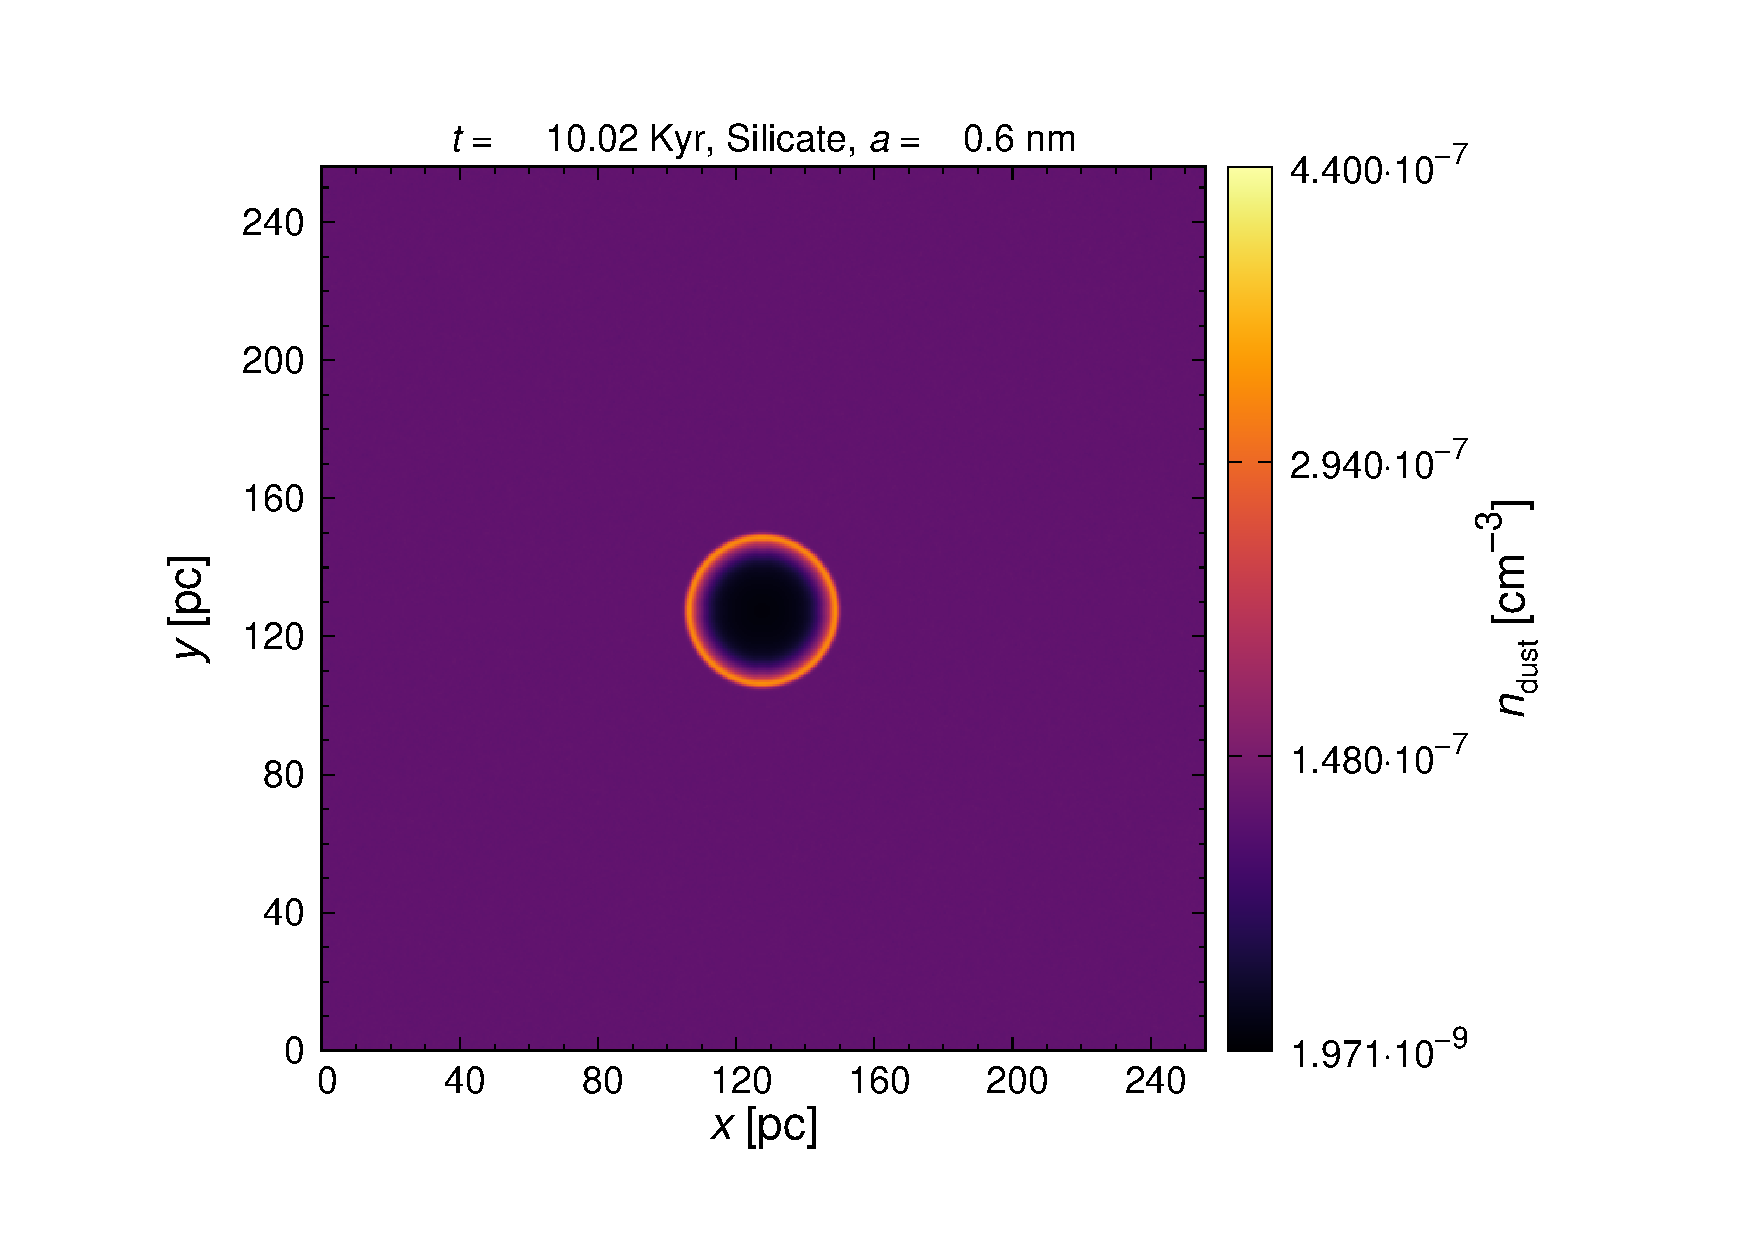
\includegraphics[trim=2.8cm 1.5cm 9.3cm 2.0cm, clip=true,page=1,height = 4.5cm]{Pics/Pics_C1/Density_1_00041.pdf}\hspace*{-0.1cm}
 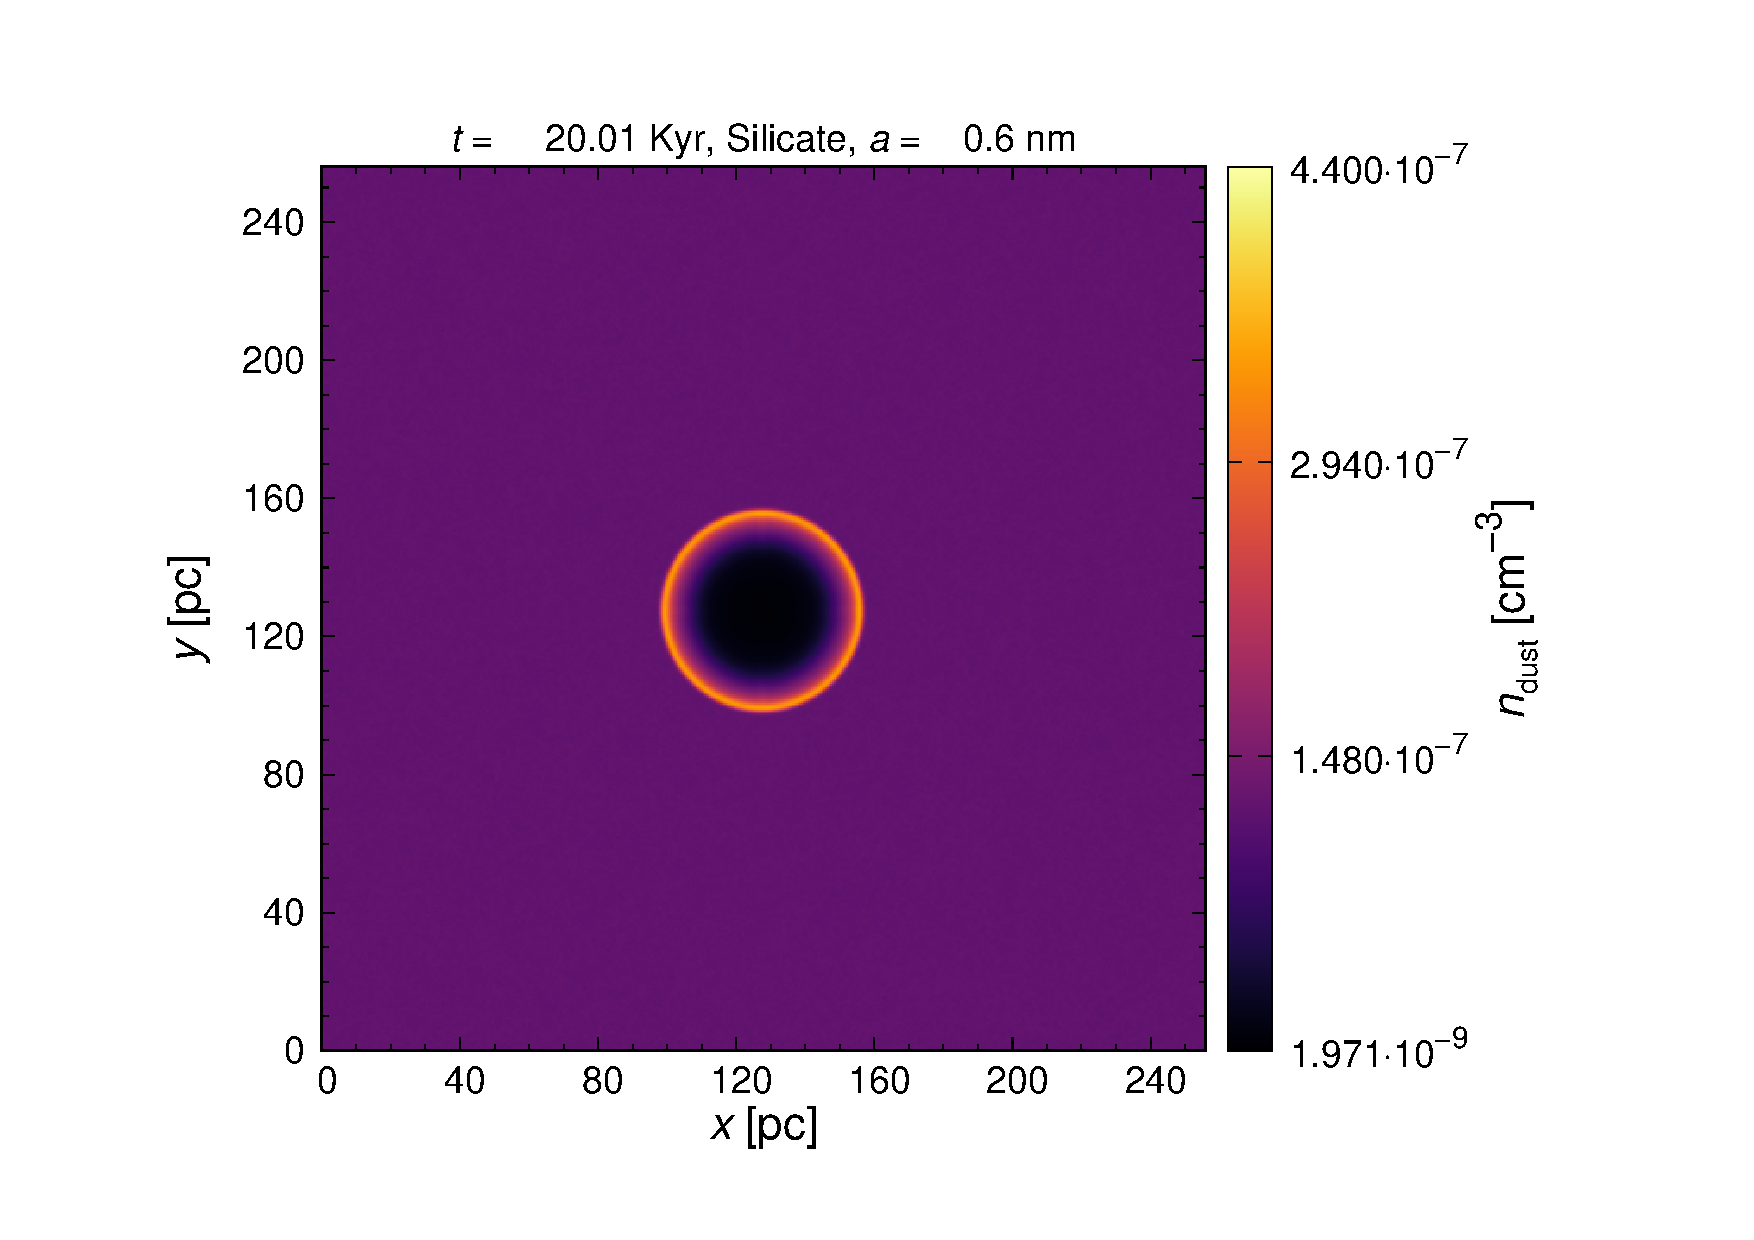
\includegraphics[trim=5.2cm 1.5cm 9.3cm 2.0cm, clip=true,page=1,height = 4.5cm]{Pics/Pics_C1/Density_1_00081.pdf}\hspace*{-0.1cm}
 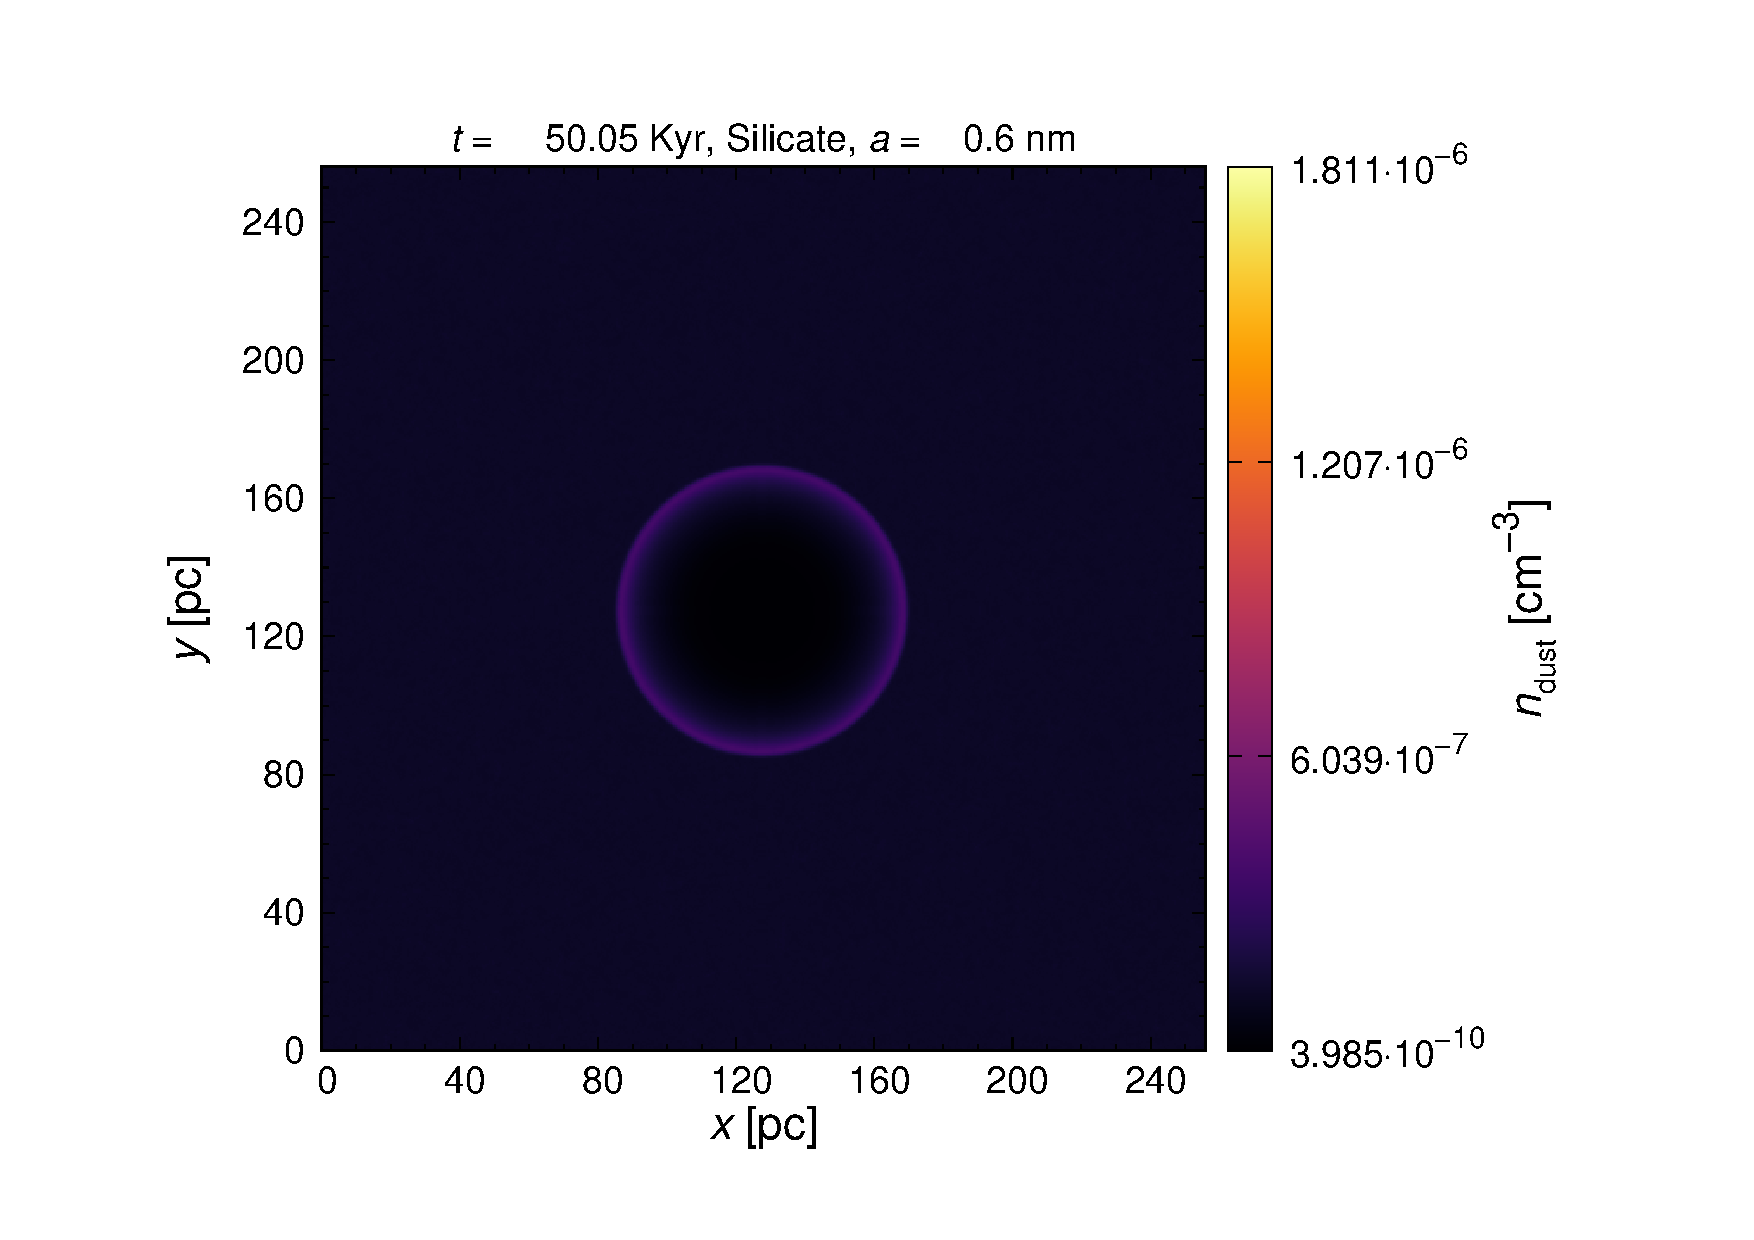
\includegraphics[trim=5.2cm 1.5cm 9.3cm 2.0cm, clip=true,page=1,height = 4.5cm]{Pics/Pics_C1/Density_1_00201.pdf}\hspace*{-0.1cm}
 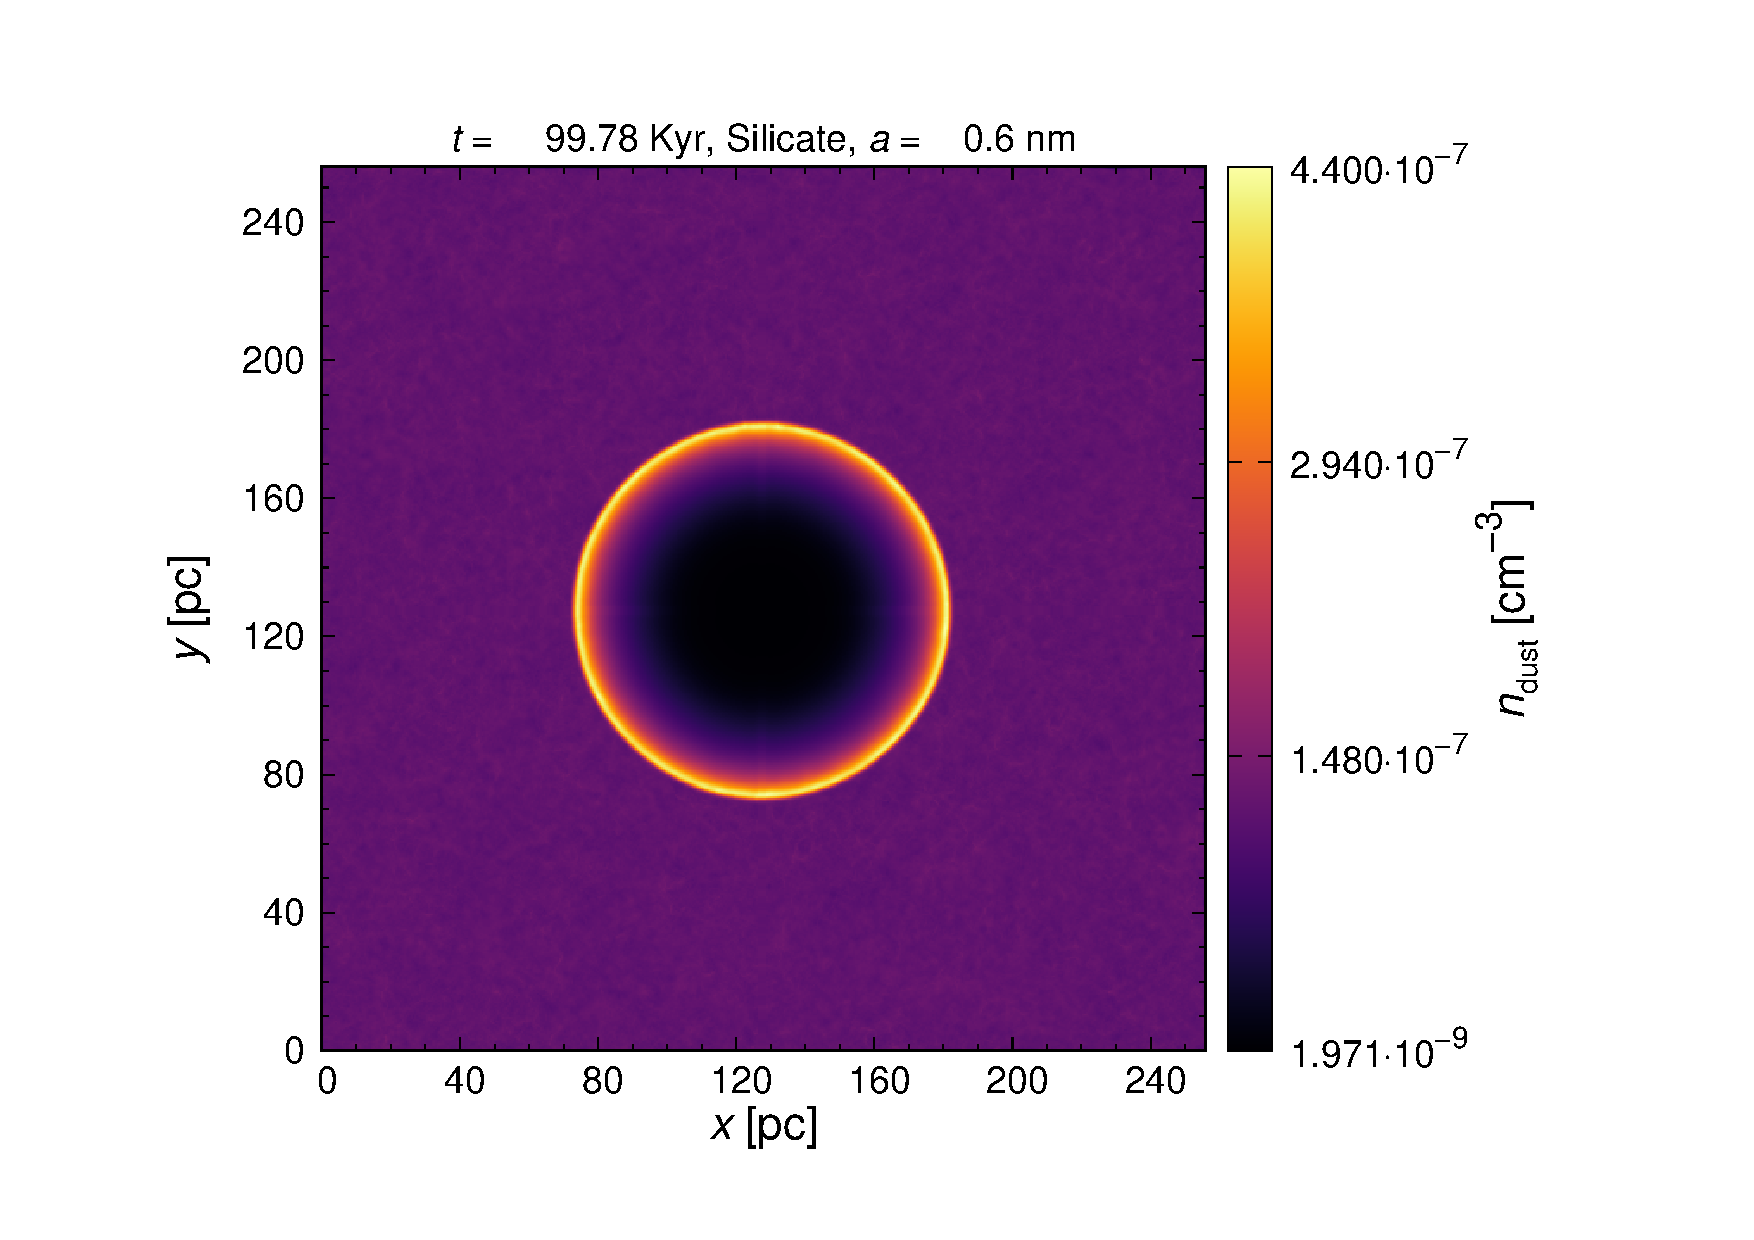
\includegraphics[trim=5.2cm 1.5cm 3.2cm 2.0cm, clip=true,page=1,height = 4.5cm]{Pics/Pics_C1/Density_1_00400.pdf}\\
  \includegraphics[trim=2.8cm 1.5cm 9.3cm 2.0cm, clip=true,page=2,height = 4.5cm]{Pics/Pics_C1/Density_1_00041.pdf}\hspace*{-0.1cm}
 \includegraphics[trim=5.2cm 1.5cm 9.3cm 2.0cm, clip=true,page=2,height = 4.5cm]{Pics/Pics_C1/Density_1_00081.pdf}\hspace*{-0.1cm}
 \includegraphics[trim=5.2cm 1.5cm 9.3cm 2.0cm, clip=true,page=2,height = 4.5cm]{Pics/Pics_C1/Density_1_00201.pdf}\hspace*{-0.1cm}
 \includegraphics[trim=5.2cm 1.5cm 3.2cm 2.0cm, clip=true,page=2,height = 4.5cm]{Pics/Pics_C1/Density_1_00400.pdf}\\
  \includegraphics[trim=2.8cm 1.5cm 9.3cm 2.0cm, clip=true,page=3,height = 4.5cm]{Pics/Pics_C1/Density_1_00041.pdf}\hspace*{-0.1cm}
 \includegraphics[trim=5.2cm 1.5cm 9.3cm 2.0cm, clip=true,page=3,height = 4.5cm]{Pics/Pics_C1/Density_1_00081.pdf}\hspace*{-0.1cm}
 \includegraphics[trim=5.2cm 1.5cm 9.3cm 2.0cm, clip=true,page=3,height = 4.5cm]{Pics/Pics_C1/Density_1_00201.pdf}\hspace*{-0.1cm}
 \includegraphics[trim=5.2cm 1.5cm 3.2cm 2.0cm, clip=true,page=3,height = 4.5cm]{Pics/Pics_C1/Density_1_00400.pdf}\\
  \includegraphics[trim=2.8cm 1.5cm 9.3cm 2.0cm, clip=true,page=4,height = 4.5cm]{Pics/Pics_C1/Density_1_00041.pdf}\hspace*{-0.1cm}
 \includegraphics[trim=5.2cm 1.5cm 9.3cm 2.0cm, clip=true,page=4,height = 4.5cm]{Pics/Pics_C1/Density_1_00081.pdf}\hspace*{-0.1cm}
 \includegraphics[trim=5.2cm 1.5cm 9.3cm 2.0cm, clip=true,page=4,height = 4.5cm]{Pics/Pics_C1/Density_1_00201.pdf}\hspace*{-0.1cm}
 \includegraphics[trim=5.2cm 1.5cm 3.2cm 2.0cm, clip=true,page=4,height = 4.5cm]{Pics/Pics_C1/Density_1_00400.pdf}\\
  \caption{Temporal evolution of the spatial dust density for \textbf{Simulation C-1} ($n_\text{gas}=0.1\,\text{cm}^{-3}$, turbulence, only dust transport). The first, second, third, and fourth rows show the distribution of 0.6, 6, 60, 600 nm grains, respectively. The colorscale is fixed for each row.}
  \end{figure*}  
 
\newpage~
\newpage~
\newpage~
\newpage
 %######################################################################################################################  %######################################################################################################################
 %###################################################################################################################### 
\section{Results and discussion}

   \begin{figure*}
        \resizebox{\hsize}{!}{
      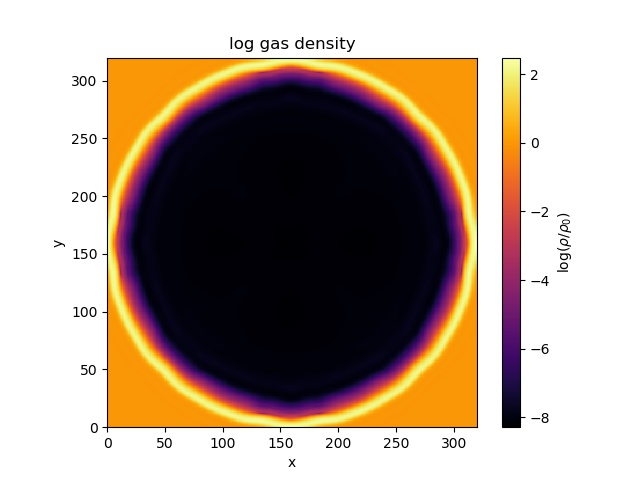
\includegraphics{3Dsedov_SN_dust_newsetup2_10pc_chi4_320_FGupd_rhoVAR60.jpg}
      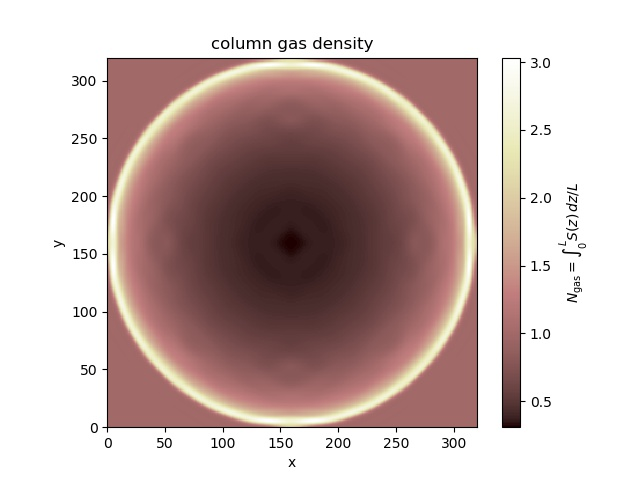
\includegraphics{3Dsedov_SN_dust_newsetup2_10pc_chi4_320_FGupd_column_gasVAR60.jpg}}
      \resizebox{\hsize}{!}{
      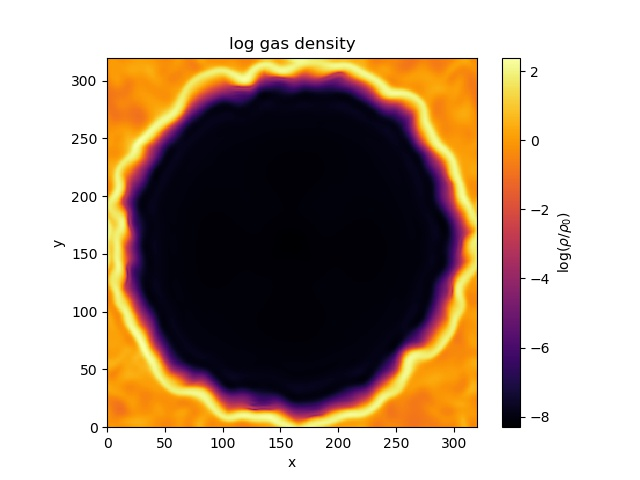
\includegraphics{3Dsedov_SN_dust_newsetup2_10pc_chi4_320_FGupd_uin2_rhoVAR60.jpg}
      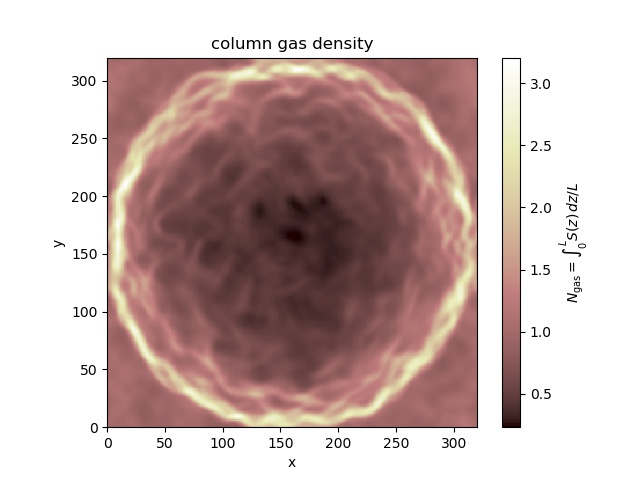
\includegraphics{3Dsedov_SN_dust_newsetup2_10pc_chi4_320_FGupd_uin2_column_gasVAR60.jpg}}

  \caption{\label{3Dsedov} }
  \end{figure*}  

  \begin{figure*}
        \resizebox{\hsize}{!}{
      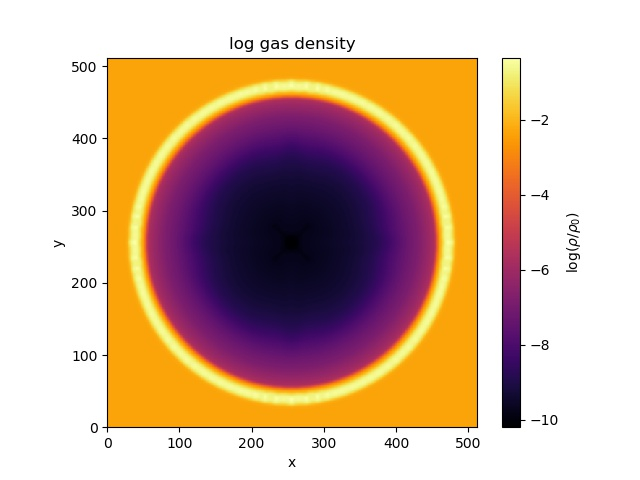
\includegraphics{3Dsedov_SN_dust_newsetup2_10pc_chi4_512_FGupd_new_n01_rhoVAR20.jpg}
      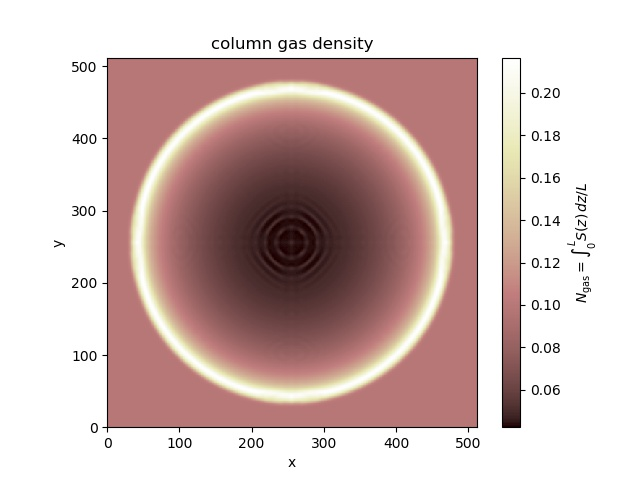
\includegraphics{3Dsedov_SN_dust_newsetup2_10pc_chi4_512_FGupd_new_n01_column_gasVAR20.jpg}}
      \resizebox{\hsize}{!}{
      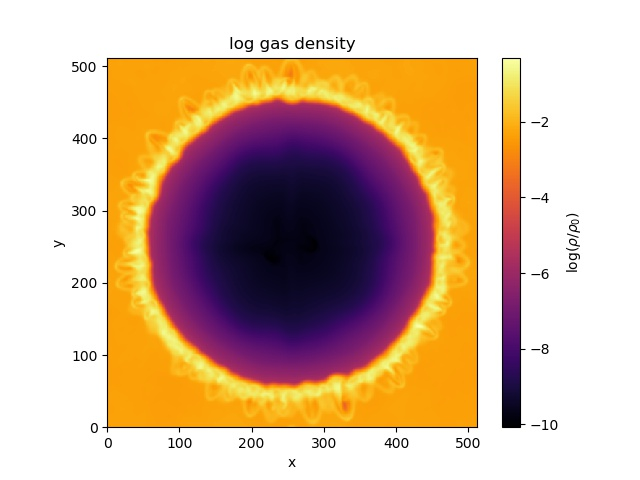
\includegraphics{3Dsedov_SN_dust_newsetup2_10pc_chi4_512_FGupd_new_n01_uin2_rhoVAR20.jpg}
      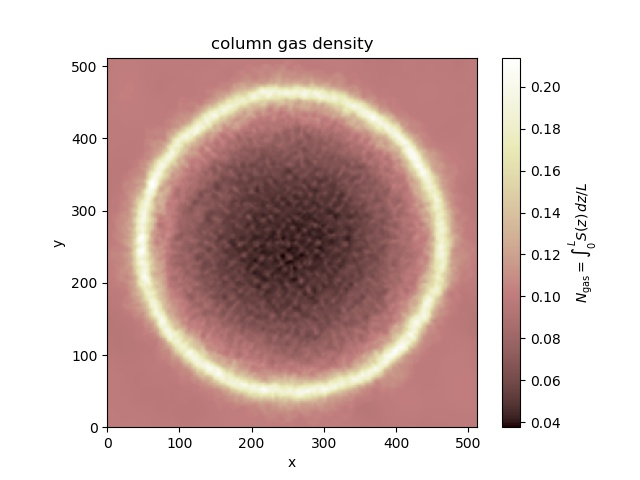
\includegraphics{3Dsedov_SN_dust_newsetup2_10pc_chi4_512_FGupd_new_n01_uin2_column_gasVAR20.jpg}}

  \caption{\label{3Dsedov} }
  \end{figure*} 

\section{Conclusions}


\section*{Acknowledgements}

The Acknowledgements section is not numbered. Here you can thank helpful
colleagues, acknowledge funding agencies, telescopes and facilities used etc.
Try to keep it short.

%%%%%%%%%%%%%%%%%%%%%%%%%%%%%%%%%%%%%%%%%%%%%%%%%%
\section*{Data Availability}

 
The inclusion of a Data Availability Statement is a requirement for articles published in MNRAS. Data Availability Statements provide a standardised format for readers to understand the availability of data underlying the research results described in the article. The statement may refer to original data generated in the course of the study or to third-party data analysed in the article. The statement should describe and provide means of access, where possible, by linking to the data or providing the required accession numbers for the relevant databases or DOIs.




%%%%%%%%%%%%%%%%%%%% REFERENCES %%%%%%%%%%%%%%%%%%

% The best way to enter references is to use BibTeX:

\bibliographystyle{mnras}
\bibliography{refs} % if your bibtex file is called example.bib


% Alternatively you could enter them by hand, like this:
% This method is tedious and prone to error if you have lots of references
%\begin{thebibliography}{99}
%\bibitem[\protect\citeauthoryear{Author}{2012}]{Author2012}
%Author A.~N., 2013, Journal of Improbable Astronomy, 1, 1
%\bibitem[\protect\citeauthoryear{Others}{2013}]{Others2013}
%Others S., 2012, Journal of Interesting Stuff, 17, 198
%\end{thebibliography}

%%%%%%%%%%%%%%%%%%%%%%%%%%%%%%%%%%%%%%%%%%%%%%%%%%

%%%%%%%%%%%%%%%%% APPENDICES %%%%%%%%%%%%%%%%%%%%%

\appendix

\section{Some extra material}

If you want to present additional material which would interrupt the flow of the main paper,
it can be placed in an Appendix which appears after the list of references.

%%%%%%%%%%%%%%%%%%%%%%%%%%%%%%%%%%%%%%%%%%%%%%%%%%


% Don't change these lines
\bsp	% typesetting comment
\label{lastpage}
\end{document}

% End of mnras_template.tex
